% Options for packages loaded elsewhere
\PassOptionsToPackage{unicode}{hyperref}
\PassOptionsToPackage{hyphens}{url}
%
\documentclass[
]{article}
\usepackage{amsmath,amssymb}
\usepackage{iftex}
\ifPDFTeX
  \usepackage[T1]{fontenc}
  \usepackage[utf8]{inputenc}
  \usepackage{textcomp} % provide euro and other symbols
\else % if luatex or xetex
  \usepackage{unicode-math} % this also loads fontspec
  \defaultfontfeatures{Scale=MatchLowercase}
  \defaultfontfeatures[\rmfamily]{Ligatures=TeX,Scale=1}
\fi
\usepackage{lmodern}
\ifPDFTeX\else
  % xetex/luatex font selection
\fi
% Use upquote if available, for straight quotes in verbatim environments
\IfFileExists{upquote.sty}{\usepackage{upquote}}{}
\IfFileExists{microtype.sty}{% use microtype if available
  \usepackage[]{microtype}
  \UseMicrotypeSet[protrusion]{basicmath} % disable protrusion for tt fonts
}{}
\makeatletter
\@ifundefined{KOMAClassName}{% if non-KOMA class
  \IfFileExists{parskip.sty}{%
    \usepackage{parskip}
  }{% else
    \setlength{\parindent}{0pt}
    \setlength{\parskip}{6pt plus 2pt minus 1pt}}
}{% if KOMA class
  \KOMAoptions{parskip=half}}
\makeatother
\usepackage{xcolor}
\usepackage[margin=1in]{geometry}
\usepackage{graphicx}
\makeatletter
\def\maxwidth{\ifdim\Gin@nat@width>\linewidth\linewidth\else\Gin@nat@width\fi}
\def\maxheight{\ifdim\Gin@nat@height>\textheight\textheight\else\Gin@nat@height\fi}
\makeatother
% Scale images if necessary, so that they will not overflow the page
% margins by default, and it is still possible to overwrite the defaults
% using explicit options in \includegraphics[width, height, ...]{}
\setkeys{Gin}{width=\maxwidth,height=\maxheight,keepaspectratio}
% Set default figure placement to htbp
\makeatletter
\def\fps@figure{htbp}
\makeatother
\setlength{\emergencystretch}{3em} % prevent overfull lines
\providecommand{\tightlist}{%
  \setlength{\itemsep}{0pt}\setlength{\parskip}{0pt}}
\setcounter{secnumdepth}{-\maxdimen} % remove section numbering
\usepackage{tikz}
\usepackage{pgfplots}
\pgfplotsset{compat=1.18}
\usetikzlibrary{shapes, positioning, calc, decorations.markings}
\newlength{\Radius}
\setlength\Radius{4em}
\usepackage{amsmath}
\usepackage{caption}
\ifLuaTeX
  \usepackage{selnolig}  % disable illegal ligatures
\fi
\IfFileExists{bookmark.sty}{\usepackage{bookmark}}{\usepackage{hyperref}}
\IfFileExists{xurl.sty}{\usepackage{xurl}}{} % add URL line breaks if available
\urlstyle{same}
\hypersetup{
  hidelinks,
  pdfcreator={LaTeX via pandoc}}

\author{}
\date{\vspace{-2.5em}}

\begin{document}

\begin{figure}
\centering
\caption*{Decomposition.}
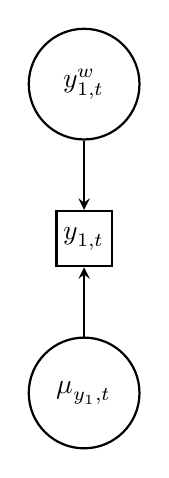
\begin{tikzpicture}[
    auto, > = latex, align=center,
    latent/.style = {circle, draw, thick, inner sep = 2pt, minimum width = \Radius},
    manifest/.style = {rectangle, draw, thick, inner sep = 0pt, minimum size = \Radius/2},
    intercept/.style = {regular polygon,regular polygon sides = 3, draw, thick, inner sep = 0pt, minimum size = \Radius},
    mean/.style = {regular polygon, regular polygon sides = 3, draw, thick, inner sep = 0pt, minimum size = 8mm},
    path/.style = {arrows = ->, thick, > = {stealth[]}},
    error/.style = {circle, draw = none, fill = none, thick, inner sep = 0pt, minimum size = 5mm},
    var/.style = {<->, thick, > = {stealth[]}, bend right = 270, looseness = 2},
    cov/.style = {<->, thick, > = {stealth[]}, bend right = 30},
    % style to add a circle in the middle of a path
    random/.style = {postaction = {decorate, decoration = {markings, mark = at position .5 with {\draw[fill = black] circle[radius = 2pt];}}}},
    ]

    \node [manifest] (y1t) {$y_{1,t}$};
    \node [latent]   (y1wt)    [above = 2.5em of y1t]  {$y_{1,t}^w$};
    \node [latent]   (mu_y1)   [below = 2.5em of y1t]  {$\mu_{y_1,t}$};

    % draw paths
    \draw [path] (y1wt) to node [] {} (y1t);
    \draw [path] (mu_y1) to node [] {} (y1t);
\end{tikzpicture}

\end{figure}
\begin{figure}
\centering
\caption*{Within-model.}
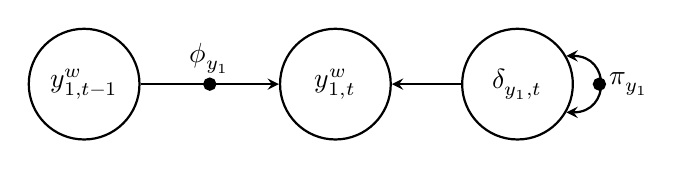
\begin{tikzpicture}[
    auto, > = latex, align=center,
    latent/.style = {circle, draw, thick, inner sep = 2pt, minimum width = \Radius},
    manifest/.style = {rectangle, draw, thick, inner sep = 0pt, minimum size = \Radius/2},
    intercept/.style = {regular polygon,regular polygon sides = 3, draw, thick, inner sep = 0pt, minimum size = \Radius},
    mean/.style = {regular polygon, regular polygon sides = 3, draw, thick, inner sep = 0pt, minimum size = 8mm},
    path/.style = {arrows = ->, thick, > = {stealth[]}},
    error/.style = {circle, draw = none, fill = none, thick, inner sep = 0pt, minimum size = 5mm},
    var/.style = {<->, thick, > = {stealth[]}, bend right = 270, looseness = 2},
    cov/.style = {<->, thick, > = {stealth[]}, bend right = 30},
    % style to add a circle in the middle of a path
    random/.style = {postaction = {decorate, decoration = {markings, mark = at position .5 with {\draw[fill = black] circle[radius = 2pt];}}}},
    ]

    % draw within-level structural model
    \node [latent] (y1wt-1)  {$y_{1,t-1}^w$};
    \node [latent] (y1wt)    [right =5em of y1wt-1]  {$y_{1,t}^w$};
    \node [latent] (delta1t)   [right =2.5em of y1wt]  {$\delta_{{y_1},t}$};

    % draw paths
    \draw [path]  (delta1t)   to node [] {}           (y1wt);
         \draw [path, postaction = random]  (y1wt-1)  to node [] {$\phi_{y_1}$}  (y1wt);
% draw (co-)variances
      \draw [var, postaction = random]    (delta1t.30)   to node [] {$\pi_{y_1}$} (delta1t.330);
\end{tikzpicture}

\end{figure}
\begin{figure}
\centering
\caption*{Between-model.}
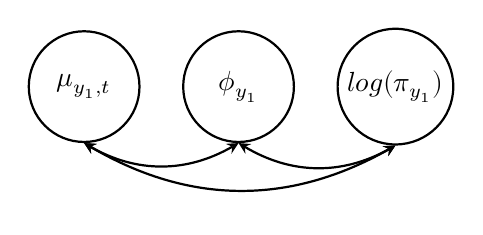
\begin{tikzpicture}[
    auto, > = latex, align=center,
    latent/.style = {circle, draw, thick, inner sep = 2pt, minimum width = \Radius},
    manifest/.style = {rectangle, draw, thick, inner sep = 0pt, minimum size = \Radius/2},
    intercept/.style = {regular polygon,regular polygon sides = 3, draw, thick, inner sep = 0pt, minimum size = \Radius},
    mean/.style = {regular polygon, regular polygon sides = 3, draw, thick, inner sep = 0pt, minimum size = 8mm},
    path/.style = {arrows = ->, thick, > = {stealth[]}},
    error/.style = {circle, draw = none, fill = none, thick, inner sep = 0pt, minimum size = 5mm},
    var/.style = {<->, thick, > = {stealth[]}, bend right = 270, looseness = 2},
    cov/.style = {<->, thick, > = {stealth[]}, bend right = 30},
    % style to add a circle in the middle of a path
    random/.style = {postaction = {decorate, decoration = {markings, mark = at position .5 with {\draw[fill = black] circle[radius = 2pt];}}}},
    ]

    % draw between-level structural model
    \node [latent] (mu_y1) {$\mu_{y_1,t}$};
    \node [latent] (phi_y1) [right = 1.5em of mu_y1] {$\phi_{y_1}$};
    \node [latent] (lnsigma2_y1) [right = 1.5em of phi_y1] {$log(\pi_{y_1})$};
    
\draw [cov] (mu_y1.south) to node [] {} (phi_y1.south);
\draw [cov] (mu_y1.south) to node [] {} (lnsigma2_y1.south);
\draw [cov] (phi_y1.south) to node [] {} (lnsigma2_y1.south);
\end{tikzpicture}

\end{figure}

\end{document}
